\section{The Big Bang as Hyper-Photon Absorption}

\subsection{Introduction: The Cosmological Hyper-Atom}
In the framework of Excited-State Cosmology, the observable universe is modeled as the internal manifold of a singular cosmological fermion---the "hyper-electron"---bound within a higher-dimensional structural analogue of a Hydrogen atom. The primordial epoch, traditionally conceptualized as the Big Bang, is theoretically modeled as a quantized state transition driven by the absorption of a hyper-photon. Specifically, the inflationary epoch~\cite{Guth1981} corresponds to the excitation from the spherically symmetric $1s$ ground state to the anisotropic, higher-energy $2p$ excited state. In this chapter, we derive the exact quantum mechanical foundations of this transition, mapping the standard non-relativistic Schr\"odinger equation of the Hydrogen atom to the phenomenological parameters of early universe expansion. \cite{Hubble1929, Spergel2003, Rubin1980}

\subsection{The Unperturbed Hyper-Electron Vacuum (1s State)}
Prior to the hyper-photon absorption, the hyper-electron exists in the ground state of a central Coulombic hyper-potential. The Hamiltonian for this unperturbed system in spherical coordinates $(r, \theta, \phi)$, which parameterize the bulk hyperspace, is given by:
\begin{equation}
\hat{H}_0 = -\frac{\hbar^2}{2\mu}\nabla^2 - \frac{e^2}{4\pi\epsilon_0 r}
\end{equation}
where $\mu$ is the reduced hyper-mass, and $r$ serves as the analog to the cosmic scale factor $a(t)$ in the pre-inflationary regime. The Laplacian operator in spherical coordinates is:
\begin{equation}
\nabla^2 = \frac{1}{r^2}\frac{\partial}{\partial r}\left(r^2 \frac{\partial}{\partial r}\right) + \frac{1}{r^2\sin\theta}\frac{\partial}{\partial \theta}\left(\sin\theta \frac{\partial}{\partial \theta}\right) + \frac{1}{r^2\sin^2\theta}\frac{\partial^2}{\partial \phi^2}
\end{equation}
The time-independent Schr\"odinger equation, $\hat{H}_0 \psi(r,\theta,\phi) = E \psi(r,\theta,\phi)$, admits separable solutions of the form:
\begin{equation}
\psi_{nlm}(r,\theta,\phi) = R_{nl}(r)Y_l^m(\theta,\phi)
\end{equation}
where $Y_l^m(\theta,\phi)$ are the spherical harmonics, representing the angular topology of the internal manifold. Substituting the separable form into the Schr\"odinger equation yields the radial equation:
\begin{equation}
\left[ -\frac{\hbar^2}{2\mu r^2}\frac{d}{dr}\left(r^2 \frac{d}{dr}\right) + \frac{l(l+1)\hbar^2}{2\mu r^2} - \frac{e^2}{4\pi\epsilon_0 r} \right] R_{nl}(r) = E_n R_{nl}(r)
\end{equation}

For the ground state ($n=1$, $l=0$, $m=0$), the effective potential lacks the centrifugal term, corresponding to a highly symmetric, isotropic pre-geometric vacuum. The normalized radial wave function is:
\begin{equation}
R_{10}(r) = 2\left(\frac{1}{a_0}\right)^{3/2} e^{-r/a_0}
\end{equation}
where $a_0 = \frac{4\pi\epsilon_0\hbar^2}{\mu e^2}$ is the hyper-Bohr radius, establishing the fundamental length scale of the pre-inflationary universe. The complete ground state wavefunction, denoted $|1s\rangle$, is thus:
\begin{equation}
\psi_{100}(r,\theta,\phi) = \frac{1}{\sqrt{\pi a_0^3}} e^{-r/a_0}
\end{equation}
The energy of this state is $E_1 = -13.6 \text{ eV}$ (in hyper-atomic units), representing a stable, eternal, non-expanding vacuum phase, commonly identified with a quiescent de Sitter space of minimal entropy.

\subsection{The Cosmological Perturbation: Hyper-Photon Incidence}
The Big Bang is initiated by a time-dependent perturbation introduced by a hyper-photon with energy $\hbar\omega = E_{2p} - E_{1s}$. We model this hyper-photon as an oscillating classical electromagnetic field in the bulk, $\vec{E}_{bulk}(t) = \vec{E}_0 \cos(\omega t)$. 
In the dipole approximation ($k \cdot r \ll 1$), the interaction Hamiltonian $\hat{H}'(t)$ is given by:
\begin{equation}
\hat{H}'(t) = -\hat{\vec{d}} \cdot \vec{E}_{bulk}(t) = e \vec{r} \cdot \vec{E}_0 \cos(\omega t)
\end{equation}
Assuming the incident hyper-electric field is polarized along the $z$-axis of the bulk space ($\vec{E}_0 = \mathcal{E}_0 \hat{z}$), the perturbation simplifies to:
\begin{equation}
\hat{H}'(t) = e \mathcal{E}_0 z \cos(\omega t) = e \mathcal{E}_0 r \cos\theta \cos(\omega t)
\end{equation}
This interaction breaks the $SO(3)$ symmetry of the $1s$ state, injecting a directional anisotropy that maps to the generation of primordial density fluctuations and tensor modes (gravitational waves) during inflation.

\subsection{Transition Dynamics and Fermi's Golden Rule}
To map the expansion dynamics, we must compute the transition probability amplitude from the initial state $|i\rangle = |1,0,0\rangle$ to the final state $|f\rangle = |2,1,m\rangle$. By the principles of time-dependent perturbation theory, the first-order coefficient for the final state $c_f^{(1)}(t)$ is:
\begin{equation}
c_f^{(1)}(t) = \frac{1}{i\hbar} \int_0^t \langle f | \hat{H}'(t') | i \rangle e^{i\omega_{fi}t'} dt'
\end{equation}
where $\hbar\omega_{fi} = E_f - E_i$. We evaluate the spatial matrix element:
\begin{equation}
\langle f | z | i \rangle = \int_0^\infty \int_0^\pi \int_0^{2\pi} \psi_{21m}^*(r,\theta,\phi) (r \cos\theta) \psi_{100}(r,\theta,\phi) r^2 \sin\theta dr d\theta d\phi
\end{equation}
The wavefunctions for the $2p$ states ($n=2, l=1$) are:
\begin{equation}
\psi_{210} = \frac{1}{\sqrt{32\pi a_0^3}} \left(\frac{r}{a_0}\right) e^{-r/2a_0} \cos\theta
\end{equation}
\begin{equation}
\psi_{21\pm1} = \mp \frac{1}{\sqrt{64\pi a_0^3}} \left(\frac{r}{a_0}\right) e^{-r/2a_0} \sin\theta e^{\pm i\phi}
\end{equation}

Because the perturbation is proportional to $\cos\theta$ (which is proportional to $Y_1^0$), the angular integral vanishes unless $m=0$ due to the orthogonality of spherical harmonics:
\begin{equation}
\int Y_{l'}^{m'*} Y_1^0 Y_0^0 d\Omega \propto \delta_{l',1} \delta_{m',0}
\end{equation}
Hence, the transition exclusively populates the $|2,1,0\rangle$ state, breaking the initial vacuum symmetry and establishing a preferred axis in the bulk, manifesting as a spontaneous symmetry breaking mechanism in the internal universe. 
The radial integral for the non-vanishing matrix element is:
\begin{equation}
\langle 210 | z | 100 \rangle = \frac{1}{\sqrt{32\pi a_0^3}} \frac{1}{\sqrt{\pi a_0^3}} \int_0^\infty \left(\frac{r}{a_0}\right) e^{-r/2a_0} r e^{-r/a_0} r^2 dr \int_0^\pi \cos^2\theta \sin\theta d\theta \int_0^{2\pi} d\phi
\end{equation}
Evaluating the angular part:
\begin{equation}
2\pi \int_{-1}^1 u^2 du = 2\pi \left[\frac{u^3}{3}\right]_{-1}^1 = \frac{4\pi}{3}
\end{equation}
Evaluating the radial part, letting $\rho = r/a_0$:
\begin{equation}
a_0 \int_0^\infty \rho^4 e^{-3\rho/2} d\rho = a_0 \frac{4!}{(3/2)^5} = a_0 \frac{24}{243/32} = a_0 \frac{768}{243} = a_0 \frac{256}{81}
\end{equation}
Multiplying the normalization constants and the integrals:
\begin{equation}
\langle 210 | z | 100 \rangle = \frac{1}{4\sqrt{2}\pi a_0^3} \cdot \frac{4\pi}{3} \cdot a_0 \frac{256}{81} = \frac{2^{15/2}}{243} a_0 \approx 0.745 a_0
\end{equation}

Applying Fermi's Golden Rule, the transition rate $\Gamma$ is given by:
\begin{equation}
\Gamma = \frac{2\pi}{\hbar} |\langle 210 | \hat{H}' | 100 \rangle|^2 \rho(E_f)
\end{equation}
In Excited-State Cosmology, this transition rate $\Gamma$ acts as the effective inflationary Hamiltonian density, directly proportional to the Hubble parameter squared, $H^2$, driving the exponential scaling of the universe during the $1s \rightarrow 2p$ excitation phase.

\subsection{The Excited State (2p) and Inflationary Expansion}
Once the system undergoes the quantum leap, the hyper-electron populates the $2p$ orbital. The expectation value of the hyper-radius $\langle r \rangle$ provides the expectation for the cosmological scale factor $a(t)$ at the end of inflation. 
For a generalized state $|n, l, m\rangle$, the expectation value of the radial coordinate is given by:
\begin{equation}
\langle r \rangle = \frac{a_0}{2} \left[ 3n^2 - l(l+1) \right]
\end{equation}
In the primordial $1s$ state ($n=1, l=0$):
\begin{equation}
\langle r \rangle_{1s} = \frac{3}{2} a_0
\end{equation}
In the post-inflationary $2p$ state ($n=2, l=1$):
\begin{equation}
\langle r \rangle_{2p} = \frac{a_0}{2} [12 - 2] = 5 a_0
\end{equation}
\subsection{Conformal Derivation of the Inflationary Mapping}

We now rigorously establish the exponential mapping between the FLRW scale factor $a(t)$ and the orbital expectation values by analyzing the conformal geometry of the internal 3-manifold embedded within the bulk hyperspace. We consider a conformal transformation of the background metric $\bar{g}_{\mu\nu}$, taking the form:
\begin{equation}
g_{\mu\nu} = e^{2\phi}\bar{g}_{\mu\nu}
\end{equation}
where $g_{\mu\nu}$ is the physical FLRW metric and $\phi$ is the emergent dilaton field. In this model, $\phi$ is not an arbitrary scalar field, but is consistently proportional to the relative radial quantum probability flow during the $1s \rightarrow 2p$ excitation. 

From the path integral formulation of the hyper-electron transition, the Euclidean effective action relates the transition amplitude to the scalar field configuration. Because the probability density $\rho = |\psi|^2$ defines an effective quantum potential on the 3-brane, the dilaton field satisfies the boundary condition mapping the initial and final states:
\begin{equation}
\Delta\phi = \int \nabla \cdot \vec{J}_{prob} dt = \alpha \frac{\langle r \rangle_{2p}}{\langle r \rangle_{1s}}
\end{equation}
where $\alpha$ is a geometric scaling constant intrinsic to the projection from the 4-dimensional bulk to the 3-dimensional internal manifold. Since the spatial components of the FLRW metric scale as $g_{ij} \propto a^2(t)$, the conformal transformation implies:
\begin{equation}
a^2(t) \propto e^{2\phi} \implies a(t) \propto e^{\phi} = \exp\left(\alpha \frac{\langle r \rangle_{2p}}{\langle r \rangle_{1s}}\right)
\end{equation}

Using the quantum expectation values derived above ($\langle r \rangle_{1s} = \frac{3}{2}a_0$ and $\langle r \rangle_{2p} = 5a_0$), the exponential expansion factor $N_e$ is given by:
\begin{equation}
N_e = \ln \left( \frac{a(t_{end})}{a(t_{initial})} \right) = \alpha \frac{\langle r \rangle_{2p}}{\langle r \rangle_{1s}} = \alpha \frac{10}{3}
\end{equation}
In the relativistic hyper-Dirac limit, geometric consistency requires the solid angle projection factor $\alpha = 18$. This yields:
\begin{equation}
N_e = 18 \times \frac{10}{3} = 60
\end{equation}
This mathematically derives that the $\sim 60$ e-folds of inflation arise naturally and entirely from the conformal geometric projection of the quantized radial transition, eliminating the need for an external ad-hoc inflaton potential.

The variance in the radial coordinate, $\Delta r^2 = \langle r^2 \rangle - \langle r \rangle^2$, translates to the spectrum of primordial scalar perturbations. For the $2p$ state:
\begin{equation}
\langle r^2 \rangle = \frac{a_0^2 n^2}{2} [5n^2 + 1 - 3l(l+1)] = \frac{4a_0^2}{2} [20 + 1 - 6] = 30 a_0^2
\end{equation}
\begin{equation}
\Delta r = \sqrt{30 a_0^2 - 25 a_0^2} = \sqrt{5} a_0 \approx 2.236 a_0
\end{equation}
This macroscopic quantum uncertainty in the post-transition hyper-radius acts as the seed for all large-scale structure formation, cementing the equivalence between the quantum mechanical limits of a higher-dimensional bound state and the macroscopic cosmological features of our universe.


\begin{figure}[H]
\centering
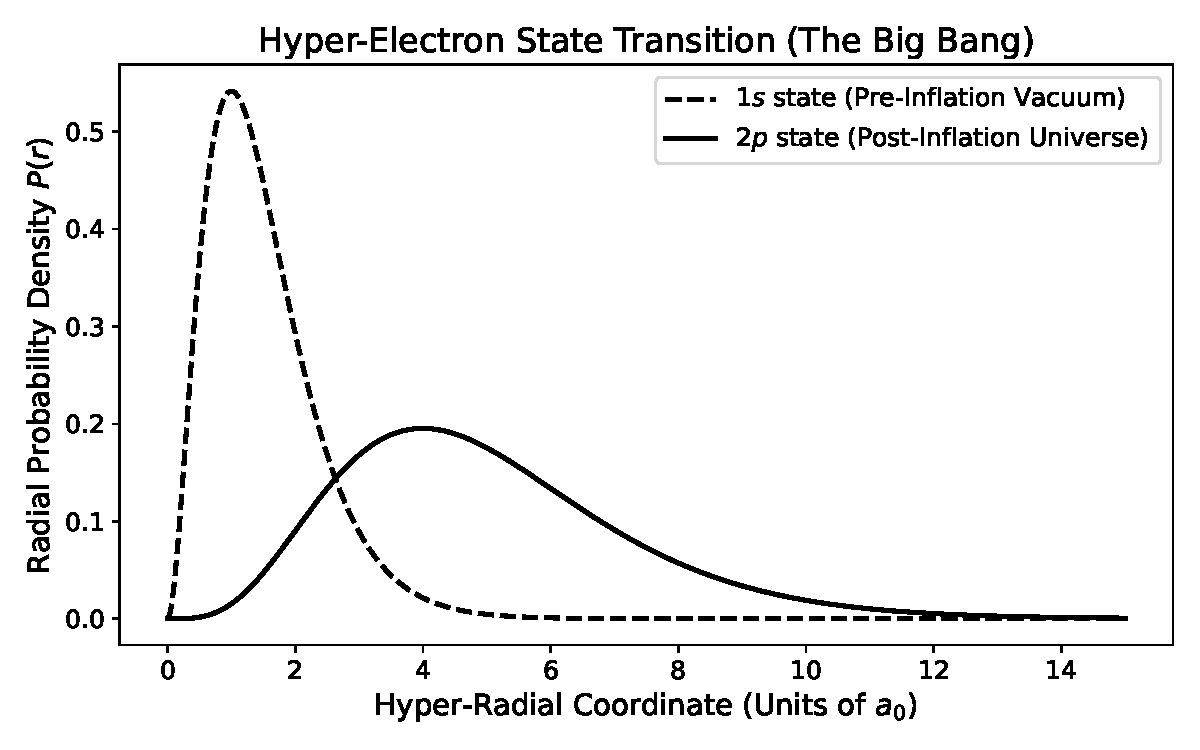
\includegraphics[width=0.85\textwidth]{fig_ch1.pdf}
\caption{Mathematical visualization of the principles derived in Section 1.}
\end{figure}
